\section{Evaluation}

\subsection{Multi-Target Linear and Multi-Class Logistic regressions}

We will start evaluating ShrinkNets with the simplest problems possible: linear
and logistic regression. As we showed, Group sparsity share similarities with
our method, this is why we will use it as baseline. We decided to focus on
multi-target linear regression because in the single target case, groups in the
Group Sparsity problem would have a size of one ($\bm{A}$ would be a vector in this
case).

The evaluation will be done on two datasets \texttt{scm1d} and \texttt{oes97}
[ref] for linear regressions and we will use \texttt{gina\_prior2} [ref] and
the \textit{Gas Sensor Array Drift Dataset} [ref] (that we shorten in
\texttt{gsadd}) for logistic regressions.

For each dataset we fit with different regularization parameters and measure
the error and sparsity obtained after convergence. In this context we define sparsity as the ratio of columns that have all their weight under $10^{-3}$ in absolute value. Parameters were choosed in
order to obtain the widest sparsity spectrum. Loss is normalized depending on the problem to be in the $[0, 1]$ range. We summarized the results in
\cref{sparsity_accuracy}. From our experiments it is clear that ShrinkNets can fit the data closer than Group Sparsity for the same amount of sparsity. The fact that we are able to reach very low loss demonstrate that even if our objective function is non convex, in practice it works as good or better as convex alternatives. Details about these datasets and the parameters used
are available in \cref{linear_datasets}.

\begin{figure}
\begin{center}
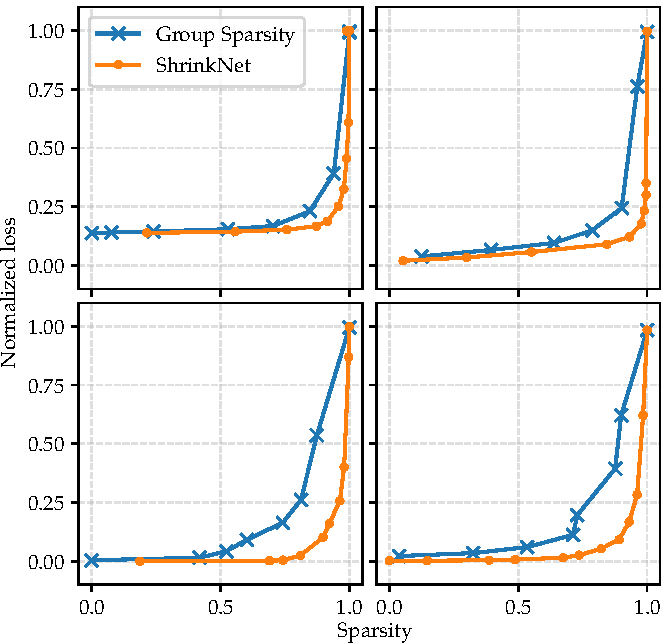
\includegraphics[width=\columnwidth]{regressions}
\vspace*{-5mm}
\caption{\label{sparsity_accuracy}Loss/Sparsity trade off comparison between Group Sparsity and Shrinknet on linear and logistic regression. From top to bottom and left to right we show the results for \texttt{scm1d}, \texttt{oes97}, \texttt{gina\_prior2} and \texttt{gsadd}.}

\end{center}
\vspace*{-4mm}
\end{figure}

\subsection{Neuron Removal strategies}

In our previous experiment, we showed that the ShrinkNet loss was
reasonable in practice, we are now interested in the impact on
early pruning. The method we suggest for early prunning uses a
parameter $\gamma$ that control the aggressiveness of neuron removal
so we will try to evaluate its impact on the final loss achieved by
the model and the cost required to train the model. Our cost model
is simple and hardware independant, we sum the number of input neurons
at each epoch. In theory the cost in time should be asymptotically
linear to this metric. To have a baseline we also train the same model
but without neuron removal. Keep in mind that this is just in order to
have some reference. Indeed, if we were to remove the neurons with small
weights it would deteriorate the loss (and picking the threshould would
be completely arbitrary). Therefore the baseline is evaluated with all neurons.
One could consider it as a "theoretical lower bound" of the best achievable loss.


We picked multiple combinations of dataset and regularization parameters ($\lambda$) and for each we fit with different aggressiveness parameters ($\gamma$). We measure the loss after convergence and the total cost and report the result in \cref{neuron_removal_figure}. In order to reduce the noise in the result, each experiment was performed $30$ times and we display the range arround $\pm$ $1$ standard deviation.

\textbf{TODO: Interpret the results}
\begin{figure}
\begin{center}
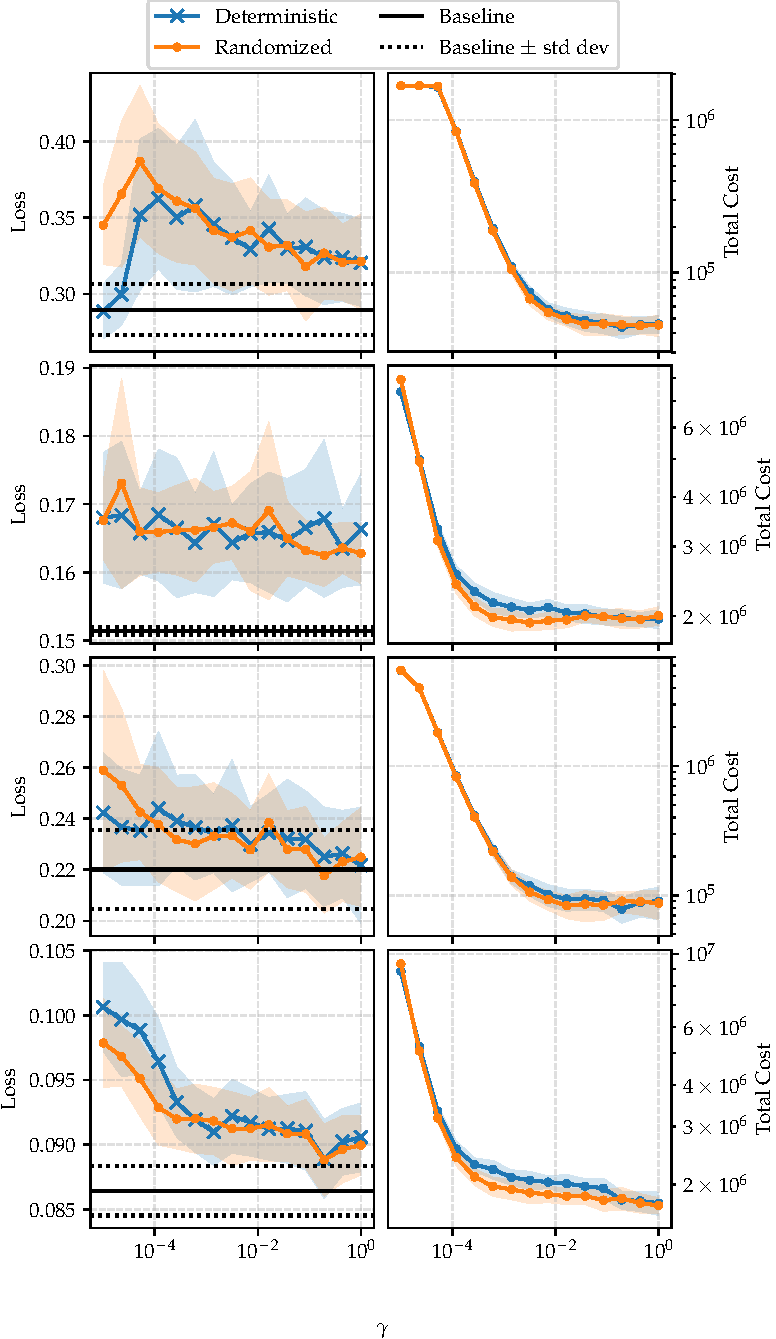
\includegraphics[width=\columnwidth]{neuron_removal}
\vspace*{-5mm}
\caption{\label{neuron_removal_figure}Effect of dynamic neuron removal for different $\gamma$. First column is the difference in the final loss in function of the removal factor. We plot theoretical baseline as a reference. Right column is a proxy of the total cost for training the model (i.e. the sum of input neurons at each epoch). Each row is a dataset/$\lambda$ combination. From top to bottom we have: \texttt{scm1d}/$0.1$, \texttt{oes97}/$0.1$}

\end{center}
\vspace*{-4mm}
\end{figure}

\subsection{Convergence and training dynamics of Neural networks}

\subsection{Hyper-optimization of ShrinkNets}

\subsection{Performance}

\section{Speeding up training with pruning}